
\marginpar{\href{https://youtu.be/19Ql_Q3l0GA}{Video}}
\marginpar{\href{https://ocw.mit.edu/courses/6-041sc-probabilistic-systems-analysis-and-applied-probability-fall-2013/pages/unit-i/lecture-3/}{Lecture Home}}
\marginpar{\href{https://ocw.mit.edu/courses/6-041sc-probabilistic-systems-analysis-and-applied-probability-fall-2013/a2015627268f4846eb3b1368623ce46f_MIT6_041SCF13_L03.pdf}{Slides}}

Experiment

\begin{figure}[ht]
\centering
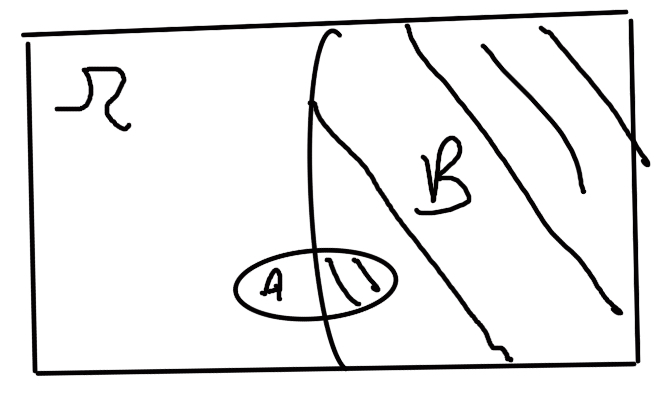
\includegraphics[width=5cm, height=4cm]{images/L03/independence.jpeg}
\caption{Independence}
\end{figure}

\begin{itemize}
    \item Outcome is in B so B is our new sample space
    \item Which A's were also assigned to B? $A \cap B$
\end{itemize}

New probabilities are conditional probabilities

\subsubsection*{Total Probability Theorem}

\begin{align*}
P(B)=P(A)P(B|A) + P(A^c)P(B|A^c)
\end{align*}

\marginpar{(4:25)} Trying to guess the state of the world based on your measurements.  That's what inference is all about.


Three Skills
\begin{itemize}
    \item Multiplication Rule - Follow tree along path
    \item Two
    \item Three
\end{itemize}

\subsection{Model Where We Toss a Coin 3 Times}

\begin{figure}[!ht]
\centering
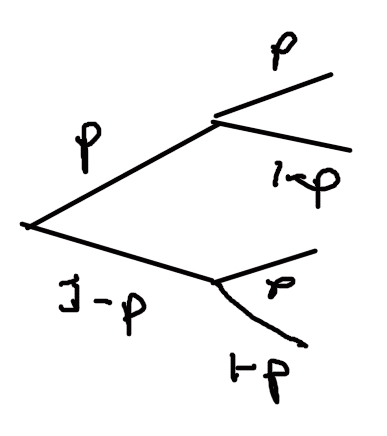
\includegraphics[width=5cm, height=4cm]{images/L03/coin_toss3.jpeg}
\caption{Coin Toss}
\end{figure}


\begin{align*}
P(H)=p, P(T)=1-p
\end{align*}

\begin{align*}
&P(THT)=(1-p)p(1-p)\\
&P(1\;Head)=3p(1-p)^2, \qquad \text{3 ways}\\
&P(\text{1st toss H}|1\;Head)=\frac{P(\text{1st toss H},1\;Head)}{P(1\;Head)}=\frac{P(HTT)}{P(1\;Head)}=\frac{p(1-p)^2}{3p(1-p)^2}=\frac{1}{3}
\end{align*}
% P(1\;Head)=3p(1-p)^2, \text{3 ways}\\
% 

\subsection{Independence}

\marginpar{(12m)}

First event gives no information for the second event.

Definition: $P(B|A)=P(B)$
$P(A \cap B)=P(A)P(B)$ This is a better definition.  It always works.
$P(A)=0 \Rightarrow independence$

\begin{figure}[ht]
\centering
\begin{tikzpicture}
\draw (0,0) rectangle (7,4);
\draw (2,2) ellipse (1cm and 1.2cm) node {A};
\draw (5,2) circle (1cm) node {B};
\end{tikzpicture}
\caption{Independent Events?} \label{fig:M22}
\end{figure}

% \begin{figure}[h]
% \centering
% \includegraphics[width=5cm, height=4cm]{IMG_1462.jpeg}
% \caption{Independent Events?}
% \end{figure}

No, separate has nothing to do with independence.  Information about A affects beliefs about B.

\subsubsection{Conditional Independence}

\marginpar{(22m)}

Definition of Conditional Independence:
\begin{align*}
P(A \cap B | C) = P(A|C)P(B|C)
\end{align*}

\marginpar{(24:00)} Independence and disjointness are two different things.

Physical link is choice of a coin.  Dependence.??

Bias coin example - see slide

\subsubsection{Independence of Collection of Events}

\marginpar{(31m)}

\begin{align*}
P(A_i \cap A_j \cap \cdots \cap A_q) = P(A_i)P(A_j)\cdots P(A_q)
\end{align*}

n=3
\begin{align*}
P(A_1 \cap A_2 \cap \cap A_3) = P(A_1)P(A_2)P(A_3)
\end{align*}

Pairwise Independence - Must apply to subcollection of events
\begin{align*}
P(A_1 \cap A_2 ) = P(A_1)P(A_2)\\
P(A_1 \cap A_3 ) = P(A_1)P(A_3)\\
P(A_2 \cap A_3 ) = P(A_2)P(A_3)\\
\end{align*}

\marginpar{(35m)} Independence and pairwise independence are two different things.

\subsubsection{Example: Pairwise but not Independent}

\begin{figure}[ht]
\centering
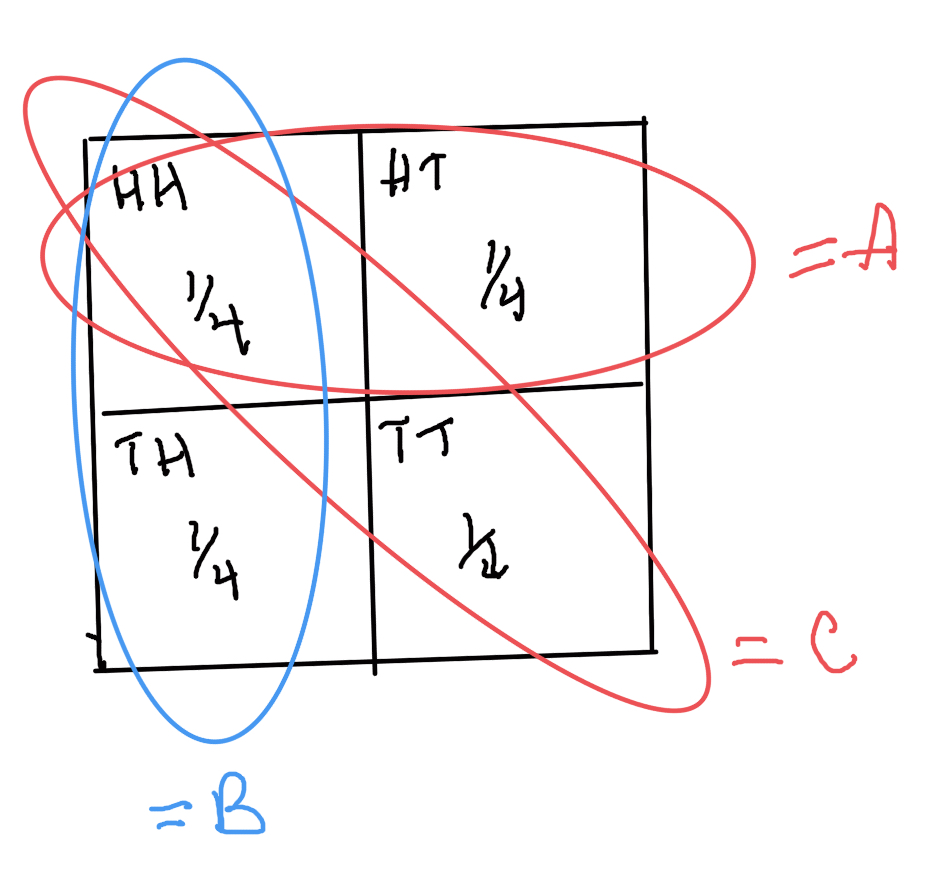
\includegraphics[width=5cm, height=4cm]{images/L03/collection_indep.jpeg}
\caption{...}
\end{figure}

They are independent mathematically:

\begin{align*}
P(A)=P(B)=\frac{1}{2}\\
\end{align*}

A={1st toss H}, B={2nd toss H}

C. First and second toss give same result

\begin{align*}
&P(C)=\frac{1}{2}\\
&P(C \cap A) = \frac{1}{4}\\
&P(A \cap B \cap C)x = \frac{1}{4}\\
&P(C|A \cap B) = 1, \qquad \text{No independence. Certain HH occurred}
\end{align*}

Therefore the three events are not independent but are pairwise independent.

\subsubsection{King's Sibling}

\marginpar{(41:25)}

\begin{figure}[ht]
\centering
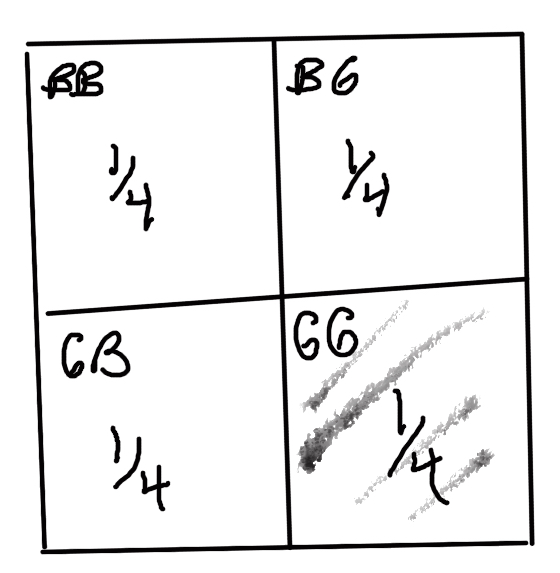
\includegraphics[width=5cm, height=4cm]{images/L03/kings_sibling.jpeg}
\caption{King's Sibling}
\end{figure}

In conditional probability $P(G)\frac{2}{3}$ (i.e. 2/3 of outcomes).

Hidden assumptions?  Things to consider: Maybe they had children until they had a boy $P(G)=1$
